\documentclass[11pt,a4paper]{article}
\usepackage{graphicx}
\usepackage{tcolorbox}
\usepackage{xcolor}
\usepackage{geometry}
\usepackage{tikz}
\usetikzlibrary{calc,arrows.meta}
\geometry{margin=0.8in}

% Define colors
\definecolor{mlblue}{RGB}{31, 119, 180}
\definecolor{mlorange}{RGB}{255, 127, 14}
\definecolor{mlgreen}{RGB}{44, 160, 44}
\definecolor{mlred}{RGB}{214, 39, 40}
\definecolor{mlpurple}{RGB}{148, 103, 189}

\title{\Large\textbf{Discovery 7: The Moving Centers}\\
\vspace{0.3em}
\normalsize Watch How Order Emerges from Chaos}
\date{}

\begin{document}
\maketitle
\vspace{-2em}

\section*{Watch the Pattern}

\begin{center}
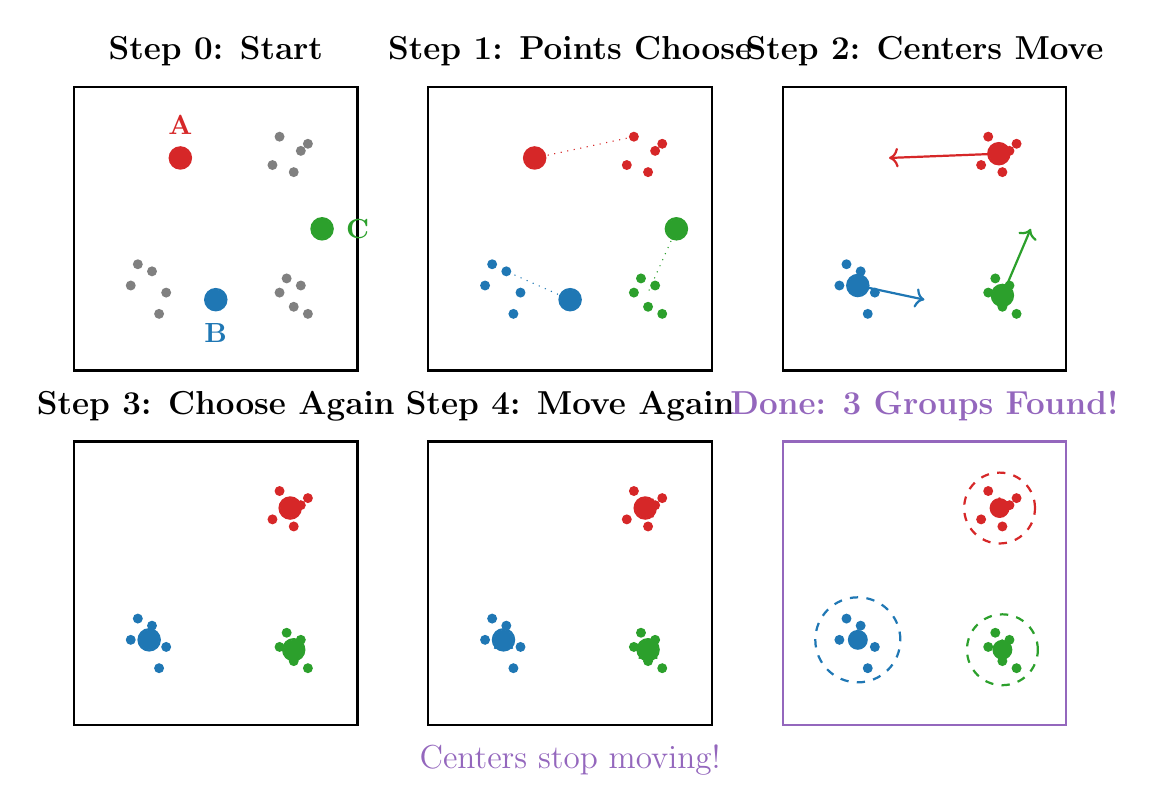
\begin{tikzpicture}[scale=0.9]
% Step 0: Random start
\begin{scope}[shift={(0,0)}]
\draw[thick] (0,0) rectangle (4,4);
\node[font=\large\bfseries] at (2,4.5) {Step 0: Start};
% Data points (fixed across all steps)
\foreach \point in {(0.8,1.2), (1.2,0.8), (0.9,1.5), (1.3,1.1), (1.1,1.4),
                    (3.2,3.1), (2.9,3.3), (3.1,2.8), (3.3,3.2), (2.8,2.9),
                    (3.2,1.2), (3.1,0.9), (2.9,1.1), (3.3,0.8), (3.0,1.3)} {
    \fill[gray] \point circle (2pt);
}
% Random initial centers
\fill[mlred] (1.5,3) circle (4pt);
\draw[mlred, thick] (1.5,3) circle (0.15);
\node[mlred, above] at (1.5,3.2) {\textbf{A}};

\fill[mlblue] (2,1) circle (4pt);
\draw[mlblue, thick] (2,1) circle (0.15);
\node[mlblue, below] at (2,0.8) {\textbf{B}};

\fill[mlgreen] (3.5,2) circle (4pt);
\draw[mlgreen, thick] (3.5,2) circle (0.15);
\node[mlgreen, right] at (3.7,2) {\textbf{C}};
\end{scope}

% Step 1: Points choose nearest center
\begin{scope}[shift={(5,0)}]
\draw[thick] (0,0) rectangle (4,4);
\node[font=\large\bfseries] at (2,4.5) {Step 1: Points Choose};
% Colored by nearest center
\foreach \point in {(0.8,1.2), (1.2,0.8), (0.9,1.5), (1.3,1.1), (1.1,1.4)} {
    \fill[mlblue] \point circle (2pt);
}
\foreach \point in {(3.2,3.1), (2.9,3.3), (3.1,2.8), (3.3,3.2), (2.8,2.9)} {
    \fill[mlred] \point circle (2pt);
}
\foreach \point in {(3.2,1.2), (3.1,0.9), (2.9,1.1), (3.3,0.8), (3.0,1.3)} {
    \fill[mlgreen] \point circle (2pt);
}
% Centers (same position)
\fill[mlred] (1.5,3) circle (4pt);
\draw[mlred, thick] (1.5,3) circle (0.15);
\fill[mlblue] (2,1) circle (4pt);
\draw[mlblue, thick] (2,1) circle (0.15);
\fill[mlgreen] (3.5,2) circle (4pt);
\draw[mlgreen, thick] (3.5,2) circle (0.15);

% Show connections
\draw[mlblue, dotted] (2,1) -- (1.1,1.4);
\draw[mlred, dotted] (1.5,3) -- (2.9,3.3);
\draw[mlgreen, dotted] (3.5,2) -- (3.1,1.1);
\end{scope}

% Step 2: Centers move to their groups
\begin{scope}[shift={(10,0)}]
\draw[thick] (0,0) rectangle (4,4);
\node[font=\large\bfseries] at (2,4.5) {Step 2: Centers Move};
% Colored points
\foreach \point in {(0.8,1.2), (1.2,0.8), (0.9,1.5), (1.3,1.1), (1.1,1.4)} {
    \fill[mlblue] \point circle (2pt);
}
\foreach \point in {(3.2,3.1), (2.9,3.3), (3.1,2.8), (3.3,3.2), (2.8,2.9)} {
    \fill[mlred] \point circle (2pt);
}
\foreach \point in {(3.2,1.2), (3.1,0.9), (2.9,1.1), (3.3,0.8), (3.0,1.3)} {
    \fill[mlgreen] \point circle (2pt);
}
% Centers moved to average
\draw[mlred, thick, <-] (1.5,3) -- (3.05,3.06);
\fill[mlred] (3.05,3.06) circle (4pt);
\draw[mlred, thick] (3.05,3.06) circle (0.15);

\draw[mlblue, thick, <-] (2,1) -- (1.06,1.2);
\fill[mlblue] (1.06,1.2) circle (4pt);
\draw[mlblue, thick] (1.06,1.2) circle (0.15);

\draw[mlgreen, thick, <-] (3.5,2) -- (3.1,1.06);
\fill[mlgreen] (3.1,1.06) circle (4pt);
\draw[mlgreen, thick] (3.1,1.06) circle (0.15);
\end{scope}

% Step 3: Points choose again
\begin{scope}[shift={(0,-5)}]
\draw[thick] (0,0) rectangle (4,4);
\node[font=\large\bfseries] at (2,4.5) {Step 3: Choose Again};
% Points now correctly grouped
\foreach \point in {(0.8,1.2), (1.2,0.8), (0.9,1.5), (1.3,1.1), (1.1,1.4)} {
    \fill[mlblue] \point circle (2pt);
}
\foreach \point in {(3.2,3.1), (2.9,3.3), (3.1,2.8), (3.3,3.2), (2.8,2.9)} {
    \fill[mlred] \point circle (2pt);
}
\foreach \point in {(3.2,1.2), (3.1,0.9), (2.9,1.1), (3.3,0.8), (3.0,1.3)} {
    \fill[mlgreen] \point circle (2pt);
}
% Centers at new positions
\fill[mlred] (3.05,3.06) circle (4pt);
\draw[mlred, thick] (3.05,3.06) circle (0.15);
\fill[mlblue] (1.06,1.2) circle (4pt);
\draw[mlblue, thick] (1.06,1.2) circle (0.15);
\fill[mlgreen] (3.1,1.06) circle (4pt);
\draw[mlgreen, thick] (3.1,1.06) circle (0.15);
\end{scope}

% Step 4: Centers move again (smaller move)
\begin{scope}[shift={(5,-5)}]
\draw[thick] (0,0) rectangle (4,4);
\node[font=\large\bfseries] at (2,4.5) {Step 4: Move Again};
% Points
\foreach \point in {(0.8,1.2), (1.2,0.8), (0.9,1.5), (1.3,1.1), (1.1,1.4)} {
    \fill[mlblue] \point circle (2pt);
}
\foreach \point in {(3.2,3.1), (2.9,3.3), (3.1,2.8), (3.3,3.2), (2.8,2.9)} {
    \fill[mlred] \point circle (2pt);
}
\foreach \point in {(3.2,1.2), (3.1,0.9), (2.9,1.1), (3.3,0.8), (3.0,1.3)} {
    \fill[mlgreen] \point circle (2pt);
}
% Very small movement
\draw[mlred, thick, <-] (3.05,3.06) -- (3.06,3.06);
\fill[mlred] (3.06,3.06) circle (4pt);
\draw[mlred, thick] (3.06,3.06) circle (0.15);

\draw[mlblue, thick, <-] (1.06,1.2) -- (1.06,1.2);
\fill[mlblue] (1.06,1.2) circle (4pt);
\draw[mlblue, thick] (1.06,1.2) circle (0.15);

\draw[mlgreen, thick, <-] (3.1,1.06) -- (3.1,1.06);
\fill[mlgreen] (3.1,1.06) circle (4pt);
\draw[mlgreen, thick] (3.1,1.06) circle (0.15);

\node[mlpurple, font=\large] at (2,-0.5) {Centers stop moving!};
\end{scope}

% Step 5: Final result
\begin{scope}[shift={(10,-5)}]
\draw[thick, mlpurple] (0,0) rectangle (4,4);
\node[font=\large\bfseries, mlpurple] at (2,4.5) {Done: 3 Groups Found!};
% Draw cluster boundaries
\draw[mlblue, thick, dashed] (1.06,1.2) circle (0.6);
\draw[mlred, thick, dashed] (3.06,3.06) circle (0.5);
\draw[mlgreen, thick, dashed] (3.1,1.06) circle (0.5);

% Final points and centers
\foreach \point in {(0.8,1.2), (1.2,0.8), (0.9,1.5), (1.3,1.1), (1.1,1.4)} {
    \fill[mlblue] \point circle (2pt);
}
\foreach \point in {(3.2,3.1), (2.9,3.3), (3.1,2.8), (3.3,3.2), (2.8,2.9)} {
    \fill[mlred] \point circle (2pt);
}
\foreach \point in {(3.2,1.2), (3.1,0.9), (2.9,1.1), (3.3,0.8), (3.0,1.3)} {
    \fill[mlgreen] \point circle (2pt);
}
\fill[mlred] (3.06,3.06) circle (4pt);
\node[mlred] at (3.06,3.06) {\textbf{*}};
\fill[mlblue] (1.06,1.2) circle (4pt);
\node[mlblue] at (1.06,1.2) {\textbf{*}};
\fill[mlgreen] (3.1,1.06) circle (4pt);
\node[mlgreen] at (3.1,1.06) {\textbf{*}};
\end{scope}
\end{tikzpicture}
\end{center}

\vspace{0.5em}

\begin{tcolorbox}[colback=mlpurple!10, colframe=mlpurple!50]
\centering\Large
\textbf{What's the pattern? Describe the dance!}
\end{tcolorbox}

\newpage

\section*{Your Turn: Predict the Moves}

\begin{center}
\Large\textbf{Where will the centers go?}

\vspace{0.5em}

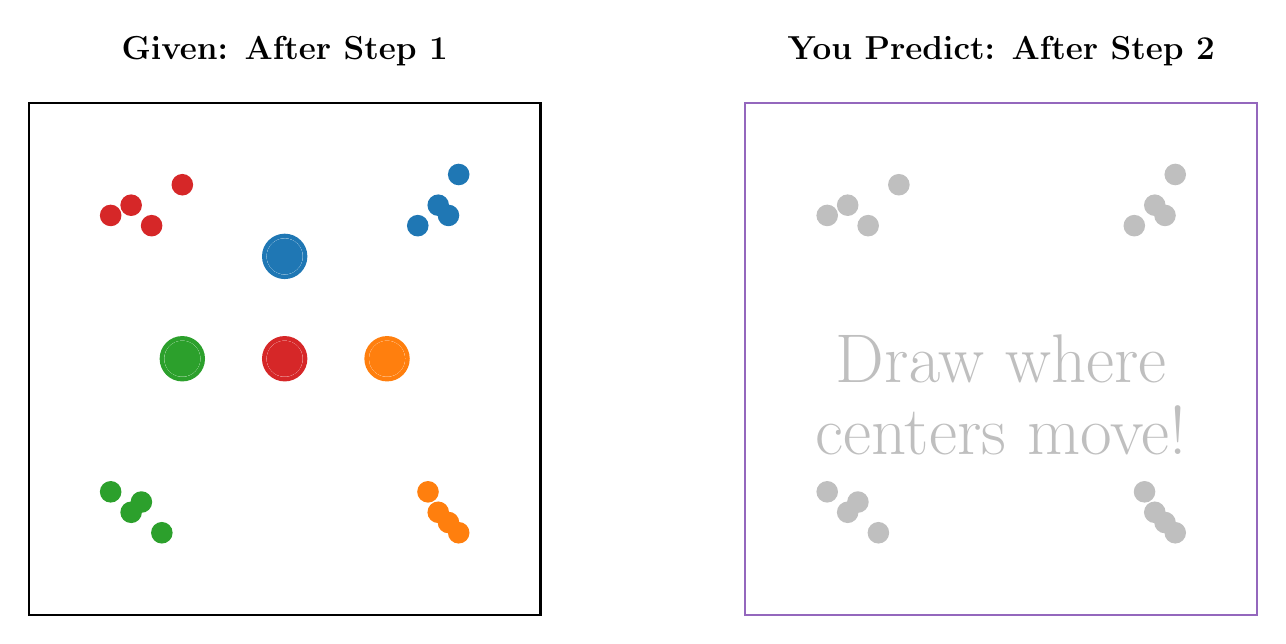
\begin{tikzpicture}[scale=1.3]
% Given situation
\begin{scope}[shift={(0,0)}]
\draw[thick] (0,0) rectangle (5,5);
\node[font=\large\bfseries] at (2.5,5.5) {Given: After Step 1};
% Data points colored
\foreach \point in {(1,4), (1.5,4.2), (1.2,3.8), (0.8,3.9)} {
    \fill[mlred] \point circle (3pt);
}
\foreach \point in {(4,4), (4.2,4.3), (3.8,3.8), (4.1,3.9)} {
    \fill[mlblue] \point circle (3pt);
}
\foreach \point in {(1,1), (1.3,0.8), (0.8,1.2), (1.1,1.1)} {
    \fill[mlgreen] \point circle (3pt);
}
\foreach \point in {(4,1), (4.2,0.8), (3.9,1.2), (4.1,0.9)} {
    \fill[mlorange] \point circle (3pt);
}
% Current center positions (wrong!)
\fill[mlred] (2.5,2.5) circle (5pt);
\draw[mlred, ultra thick] (2.5,2.5) circle (0.2);
\node[mlred] at (2.5,2.5) {\textbf{A}};

\fill[mlblue] (2.5,3.5) circle (5pt);
\draw[mlblue, ultra thick] (2.5,3.5) circle (0.2);
\node[mlblue] at (2.5,3.5) {\textbf{B}};

\fill[mlgreen] (1.5,2.5) circle (5pt);
\draw[mlgreen, ultra thick] (1.5,2.5) circle (0.2);
\node[mlgreen] at (1.5,2.5) {\textbf{C}};

\fill[mlorange] (3.5,2.5) circle (5pt);
\draw[mlorange, ultra thick] (3.5,2.5) circle (0.2);
\node[mlorange] at (3.5,2.5) {\textbf{D}};
\end{scope}

% Space for prediction
\begin{scope}[shift={(7,0)}]
\draw[thick, mlpurple] (0,0) rectangle (5,5);
\node[font=\large\bfseries] at (2.5,5.5) {You Predict: After Step 2};
% Same data points (gray)
\foreach \point in {(1,4), (1.5,4.2), (1.2,3.8), (0.8,3.9),
                    (4,4), (4.2,4.3), (3.8,3.8), (4.1,3.9),
                    (1,1), (1.3,0.8), (0.8,1.2), (1.1,1.1),
                    (4,1), (4.2,0.8), (3.9,1.2), (4.1,0.9)} {
    \fill[gray!50] \point circle (3pt);
}
\node[gray!50] at (2.5,2.5) {\Huge Draw where};
\node[gray!50] at (2.5,1.8) {\Huge centers move!};
\end{scope}
\end{tikzpicture}

\vspace{1em}

\textbf{The Rule:} \underline{\hspace{10cm}}

\underline{\hspace{14cm}}
\end{center}

\vspace{1em}

\section*{Discovery Questions}

\begin{center}
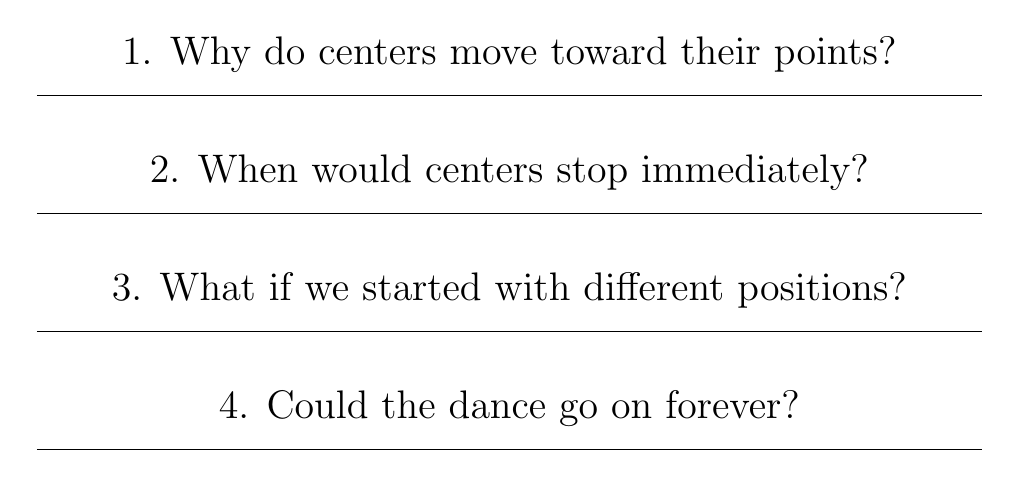
\begin{tikzpicture}[scale=1]
\node[font=\Large] at (0,0) {1. Why do centers move toward their points?};
\node at (0,-0.5) {\underline{\hspace{12cm}}};

\node[font=\Large] at (0,-1.5) {2. When would centers stop immediately?};
\node at (0,-2) {\underline{\hspace{12cm}}};

\node[font=\Large] at (0,-3) {3. What if we started with different positions?};
\node at (0,-3.5) {\underline{\hspace{12cm}}};

\node[font=\Large] at (0,-4.5) {4. Could the dance go on forever?};
\node at (0,-5) {\underline{\hspace{12cm}}};
\end{tikzpicture}
\end{center}

\vspace{1em}

\section*{The Big Idea}

\begin{center}
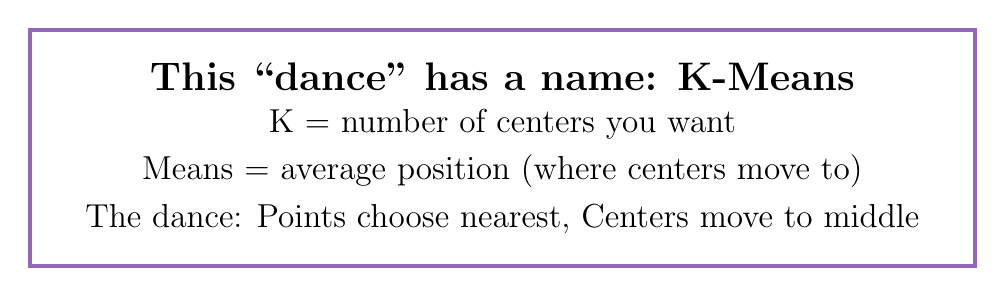
\begin{tikzpicture}[scale=1.2]
\draw[ultra thick, mlpurple] (0,0) rectangle (10,2.5);

\node at (5,2) {\Large\textbf{This ``dance'' has a name: K-Means}};
\node at (5,1.5) {\large K = number of centers you want};
\node at (5,1) {\large Means = average position (where centers move to)};
\node at (5,0.5) {\large The dance: Points choose nearest, Centers move to middle};
\end{tikzpicture}
\end{center}

\vspace{0.5em}

\begin{tcolorbox}[colback=mlblue!10, colframe=mlblue!50]
\centering\large
\textbf{Next Class:} See this dance with thousands of points!
\end{tcolorbox}

\end{document}